\documentclass{article} 
\usepackage{beamerarticle}

%\documentclass[ignorenonframetext]{beamer} 
%\usetheme{Warsaw}
%\usepackage{lipsum}

\usepackage{hyperref}
\usepackage[references,links]{agda}
\usepackage{amsmath}
\usepackage{amsthm}
\usepackage{mathtools}
\usepackage{textgreek}
\usepackage{catchfilebetweentags}
\usepackage{tipa}
\usepackage{graphicx}
\usepackage{bussproofs}
\usepackage{tikz}

%math
\newcommand{\alp}{\ensuremath{\alpha}}
\newcommand{\lamb}{\ensuremath{\lambda}}
\newcommand{\alpsym}{\ensuremath{\sim_\alpha}}
\newcommand{\choice}{\ensuremath{\chi}}
\newcommand{\p}{\ensuremath{\rightrightarrows}}
\newcommand{\ninb}{\ensuremath{\not\in_b}}

%Agda
\newcommand{\freshin}[2]{\ensuremath{#1 \mathbin{\AgdaDatatype{\#}} #2}}
\newcommand{\lambAg}[2]{\ensuremath{\AgdaInductiveConstructor{ƛ}\, #1\, #2}}
\newcommand{\inAg}{\ensuremath{\mathbin{\AgdaFunction{∈}}}}
\newcommand{\ninAg}{\ensuremath{\mathbin{\AgdaFunction{∉}}}}
\newcommand{\neqAg}{\ensuremath{\mathbin{\AgdaInductiveConstructor{≢}}}}
\newcommand{\ap}[2]{#1 \ensuremath{\mathbin{\AgdaInductiveConstructorFunction{·}} #2}}
\newcommand{\var}[1]{\ensuremath{\AgdaInductiveConstructorFunction{v}\, #1}}
\newcommand{\fv}{\ensuremath{{\AgdaFunction{fv}}\,}}
\newcommand{\perm}{\ensuremath{\mathbin{\AgdaFunction{∙}}}}
\newcommand{\perma}{\ensuremath{\mathbin{\AgdaFunction{∙}_a}}}
\newcommand{\free}{\ensuremath{\mathbin{\AgdaFunction{*}}}}
\newcommand{\choiceAg}{\ensuremath{\AgdaFunction{χ}\,}}
\newcommand{\choiceAgaux}{\ensuremath{\AgdaFunction{χ'}\,}}
\newcommand{\alpeqAg}{\ensuremath{\mathbin{\AgdaDatatype{∼α}}}}
\newcommand{\swap}[3]{\ensuremath{(#1 \mathbin{\AgdaFunction{∙}} #2)\, #3}}

\newcommand{\betaalpha}{\ensuremath{\rightarrow_\alpha}}
\newcommand{\betaaster}{\ensuremath{\rightarrow_\beta^*}}
\newcommand{\lam}{\ensuremath{\lambda}}
\newcommand{\conc}{\ensuremath{\mathop{+\!\!+}}}


% \newcommand{\agdaf}[1]{\ensuremath{\AgdaFunction{#1}\,}}
% \newcommand{\agdaD}[1]{\ensuremath{\AgdaDatatype{#1}\,}}
% \newcommand{\agdav}[1]{\ensuremath{\AgdaBound{#1}\,}}

\DeclareUnicodeCharacter{411}{\textipa{\textcrlambda}}
\DeclareUnicodeCharacter{65288}{(}
\DeclareUnicodeCharacter{65289}{)}
\DeclareUnicodeCharacter{8788}{\ensuremath{\coloneqq}}
\DeclareUnicodeCharacter{8336}{\ensuremath{_a}}
\DeclareUnicodeCharacter{8799}{\ensuremath{\overset{?}{=}}}
\DeclareUnicodeCharacter{8759}{\ensuremath{\dblcolon}}
\DeclareUnicodeCharacter{8718}{\ensuremath{\square}}

\newtheorem{lem}{Lemma}

\begin{document}


\section{Alpha Conversion}\label{alpha}


\begin{frame}

\mode<presentation>{
  \begin{block}{Alpha Conversion}
  \end{block}
}


\begin{minipage}{0.4\linewidth}
  \AxiomC{$$} \LeftLabel{\alpsym v} \UnaryInfC{$x \alpsym x$} \DisplayProof
\end{minipage}
\begin{minipage}{0.4\linewidth}
  \AxiomC{$M \alpsym M'$} 
  \AxiomC{$N \alpsym N'$}
  \LeftLabel{\alpsym a}
  \BinaryInfC{$M N \alpsym M' N'$} \DisplayProof
\end{minipage}
\begin{minipage}{0.4\linewidth}
  \AxiomC{$\exists xs, \forall z \not\in xs, (x\ z) M \alpsym (y\ z) N$} 
    \LeftLabel{\alpsym \lam}
  \UnaryInfC{$\lambda x M  \alpsym  \lambda y N$} \DisplayProof
\end{minipage}

\section{Parallel Reduction}\label{parallel}

\mode<presentation>{
  \begin{block}{Parallel Reduction}
  \end{block}
}

\begin{minipage}{0.4\linewidth}
  \AxiomC{$$}   \LeftLabel{\p v} \UnaryInfC{$x \p x$} \DisplayProof
\end{minipage}
\begin{minipage}{0.4\linewidth}
  \AxiomC{$M \p M'$} 
  \AxiomC{$N \p N'$}
  \LeftLabel{\p a}
  \BinaryInfC{$M N \p M' N'$} \DisplayProof
\end{minipage}
\begin{minipage}{0.4\linewidth}
  \AxiomC{$\exists xs, \forall z \not\in xs, (x\ z) M \p (y\ z) N$} 
  \LeftLabel{\p \lam}
  \UnaryInfC{$\lambda x M  \p  \lambda y N$} \DisplayProof
\end{minipage}

\begin{center}
  \AxiomC{$\lambda x M \p \lambda y P'$}
  \AxiomC{$N \p  P''$}
  \AxiomC{$ P' [y := P''] \alpsym P$}
  \LeftLabel{$\p \beta$}
  \TrinaryInfC{$(\lambda x M) N  \p P$}
  \DisplayProof
\end{center}


\end{frame}

\begin{frame}

\section{New Substitution Lemmas}
\begin{lem}[Swapping substitution variable]
\label{pequiv}
\[ x \# M  \Rightarrow ((x\ y) M) [x:=N] \alpsym  M [y := N] \]
\end{lem}

\mode<presentation>{
Proof uses \alp-induction principle.
}
% \mode
% <all> 


\end{frame}
  
\begin{proof} 
Uses \alp-induction principle on $M$\ term to avoid $x,y$\ and the free variables in $N$ as binder position in the \lam-case.

For some arbitrary $x,y$\ variables and term $N$\ we define the following predicate over terms:

\[ P(M) \equiv x \# M \Rightarrow  (x\ y) M [x:=N] \alpsym  M [y := N] \]

We prove $P$\ is \alp-compatible, given $N$\ such that $M \alpsym P$\ and $P(M)$ we prove $P(P)$\ holds. As $x \# P$\ and $P \alpsym M$\ then $x \# M$, then: 

\[
\begin{array}{ccl}
         (( x\ y) P) [ x := N ] &\equiv& \{\text{\alp\ equiv. and subst. lemma} \}\\
         ((x\ y) M) [ x :=  N ] &\alpsym& \{ \text{as } x \# M\ \text{we can apply}\ P(M) \}\\
         M [ y ≔ N ] &\equiv& \{\text{subst. lemma}\} \\ 
         P [ y ≔ N ]
\end{array}
\]

  \begin{itemize}
  \item [var case:] Hypotheses: $x \# z$ Thesis: $((x\ y)z) [x := N] \alpsym z [ y := N]$

    As $x \# z$\ then $x \not= z$.

    \begin{itemize}
    \item[$y = z$\ case:] $((x\ y)y) [x := N] =  x [x := N] = N = y [y := N]$
    \item[$y\not= z$\ case:] $((x\ y)z) [x := N] =  z [x := N] = z = z [y := N]$
    \end{itemize}
  \item [app. case:] Hypotheses: $x \# M P $ Thesis: $((x\ y) (M P)) [x := N] \alpsym (M P) [ y := N]$
    
    \[ \begin{array}{ccl}
      ((x\ y) (M P)) [x := N] &=& \\
      (((x\ y) M) ((x\ y)P)) [x := N] &=& \\
      (((x\ y) M) [x := N]) (((x\ y)P)[x := N])  &\alpsym& \{\text{ih}\}\\
      (M [y := N]) (P[y := N])  &=& \\
      (M P) [y := N]
    \end{array} \]

  \item [\lam\ case:] Hypotheses: $x \# \lam z M \wedge z \not\in \{x,y\} \cup fv(N)$ \\
                      Thesis: $((x\ y) (\lam z M )) [x := N] \alpsym (\lam z M) [ y := N]$ \\
     As $z \not\in \{x,y\} \cup fv(N)$\ then $z \not= x$. Because $x \# \lam z M$\ and $z \not=x$\ then $x \# M$.


    \[ \begin{array}{ccl}
      ((x\ y) (\lam z M)) [x := N] &=& \\
      (\lam ((x\ y) z) ((x\ y) M)) [x := N] &=& \{ z \not\in \{x,y\} \cup fv(N) \}\\
      (\lam z ((x\ y) M)) [x := N] &\alpsym& \{ z \not\in \{x,y\} \cup fv(N) \} \\
      \lam z (((x\ y) M) [x := N])  &\alpsym& \{\text{ih}\}\\
      \lam z (M [y := N])  &\alpsym& \{ z \not\in \{x,y\} \cup fv(N) \} \\
      (\lam z M)  [y := N]
    \end{array} \]
    
  \end{itemize}

\end{proof}

\begin{lem}[Substitution preserves freshness (no capture lemma)]
\label{nocapture}
\[ x \# \lam y M   \wedge x \# N \Rightarrow x \# M [ y := N] \]
\end{lem}


\begin{proof} Uses \alp-induction principle on $M$\ term to avoid $x,y$\ and the free variables in $N$ as binder position in the \lam-case.

  \begin{itemize}
  \item[var case $(M=z)$:] Hypothesis: $x \# \lam y z \wedge x \# N$ Thesis:  $x \# z [y := N]$
    \begin{itemize}
    \item[$y = z$ case:] Then $z [y:=N] = y [y := N] = N$, as $x \# N$\ by hypothesis, $x \# z [y := N]$.
    \item[$y \not= z$ case:] $z [y:=N] = z$ so we have to prove that $x \not= z$. As $x \# \lam y z$\ then $x = y$\ or the desired result $x \not= z$. Finally, for the pending case, if $x = y$\ as $y \not= z$ then $x \not= z$.
    \end{itemize}

  \item[app. case $(M=P Q)$:] Hypothesis: $x \# \lam y (P Q) \wedge x \# N$ Thesis: $x \# (P Q) [y := N]$
    
    \AxiomC{$x \# \lam y (P Q)$}
    \UnaryInfC{$x \# \lam y P \wedge x \# \lam y P$}
    \AxiomC{$x \# N$}
    \LeftLabel{ih}
    \BinaryInfC{$x \# P [x := N] \wedge x \# Q [x:=N]$}
    \LeftLabel{$\#$a}
    \UnaryInfC{$x \# (P [x := N]) (Q [x := N]) = (P Q) [x := N]$}
    \DisplayProof

  \item[\lam\ case $(M=\lam z M)$:] Hypothesis: $z \not\in \{x,y\} \cup fv(N) \wedge x \# \lam y (\lam z M) \wedge x \# N$ \\ Thesis: $x \# (\lam z M) [y := N]$

  \AxiomC{$z \not= x$}
  \AxiomC{$x \# \lam y (\lam z M)$}    
  \BinaryInfC{$x \# \lam y M$}
  \AxiomC{$x \# N$}
  \LeftLabel{ih}
  \BinaryInfC{$x \# M [y := N]$}
  \UnaryInfC{$x \# \lam z (M [y := N])$}
  \AxiomC{$z \not\in fv(N)$}
  \UnaryInfC{$z \# M$}
  \UnaryInfC{$\lam z (M [y := N]) \alpsym (\lam z M) [y := N]$}
  \BinaryInfC{$x \# (\lam z M) [y := N]$}
  \DisplayProof
  \end{itemize}

\end{proof}


\section{Parallel Relation Lemmas}

\begin{lem}[Parallel is equivariant]
\label{pequiv}
\[ M \p N \Rightarrow \pi M \p \pi N \]
\end{lem}

\begin{proof}
Induction on the parallel relation.

\begin{itemize}
   \item[var. rule:] Direct.
   \item[app. rule:] Direct.
   \item[\lam\ rule:] 
\begin{minipage}{0.2\linewidth}
     Hypotheses:
\end{minipage}
\begin{minipage}{0.4\linewidth}
  \AxiomC{$\exists xs, \forall z \not\in xs, (x\ z) M \p (y\ z) N$} 
  \LeftLabel{\p \lam}
  \UnaryInfC{$\lambda x M  \p  \lambda y N$} \DisplayProof
\end{minipage}

Thesis:  $\lambda (\pi\ x) (\pi\ M)  \p  \lambda (\pi\ y) (\pi\ N)$

Proof:


  \AxiomC{$\exists xs, \forall z \not\in xs, (x\ z) M \p (y\ z) N$} 
  \UnaryInfC{$\forall z \not\in xs \conc dom(\pi), (x\ z) M \p (y\ z) N$} 
  \LeftLabel{ih}
  \UnaryInfC{$\forall z \not\in xs \conc dom(\pi), \pi ((x\ z) M) \p \pi ((y\ z) N)$} 
  \UnaryInfC{$\forall z \not\in xs \conc dom(\pi),  ((\pi\ x)\ (\pi\ z)) (\pi\ M) \p  ((\pi\ y)\ (\pi\ z)) (\pi\ N)$} 
  \LeftLabel{$(\pi\ z) \equiv z\ as\ z \not\in dom(\pi) $}
  \UnaryInfC{$ \forall z \not\in xs \conc dom(\pi), ((\pi\ x)\ z) (\pi\ M) \p ((\pi\ y)\ z) (\pi\ N)$} 
  \LeftLabel{\p \lam}
  \UnaryInfC{$\lambda (\pi\ x) (\pi\ M)  \p  \lambda (\pi\ y) (\pi\ N)$} \DisplayProof


   \item[$\beta$\ rule:]
\begin{minipage}{0.2\linewidth}
     Hypotheses:
\end{minipage}
\begin{minipage}{0.4\linewidth}
  \AxiomC{$\lambda x M \p \lambda y P'$}
  \AxiomC{$N \p  P''$}
  \AxiomC{$P \alpsym P' [y := P'']$}
  \LeftLabel{$\p \beta$}
  \TrinaryInfC{$(\lambda x M) N  \p P$}
  \DisplayProof
\end{minipage}

Thesis:  $(\lambda (\pi\ x) (\pi\ M)) (\pi\ N)  \p \pi\ P$

Proof:
  \AxiomC{$\lambda x M \p \lambda y P'$}
  \LeftLabel{ih}
  \UnaryInfC{$\lambda (\pi\ x) (\pi\ M) \p \lambda (\pi\ y) (\pi\ P')$}
  \AxiomC{$N \p  P''$}
  \LeftLabel{ih}
  \UnaryInfC{$\pi\ N \p  \pi\ P''$}
  \AxiomC{$P \alpsym P' [y := P'']$}
  \LeftLabel{\alp\ equiv.}
  \UnaryInfC{$\pi\ P \alpsym \pi\ (P' [y := P''])$}
  \LeftLabel{\alp\ ind.}
  \UnaryInfC{$\pi\ P \alpsym (\pi\ P') [ (\pi\ y) := (\pi\ P'')]$}
  \LeftLabel{$\p \beta$}
  \TrinaryInfC{$(\lambda (\pi\ x) (\pi\ M)) (\pi\ N)  \p \pi\ P$}
  \DisplayProof
\end{itemize}
\end{proof}

\begin{lem}[Parallel is right \alp-equivalent]
\label{prightalpha}
\[ M \p N \wedge N \alpsym P \Rightarrow M \p P \]
\end{lem}

\begin{proof}
Trivial induction on the parallel relation.

\begin{itemize}
   \item[var. rule:] Direct.
   \item[app. rule:] Direct.
   \item[\lam\ rule:] 

     Hypotheses: 

\begin{minipage}{0.5\linewidth}
  \AxiomC{$\exists xs, \forall z \not\in xs, (x\ z) M \p (y\ z) N$} 
  \LeftLabel{\p \lam}
  \UnaryInfC{$\lambda x M  \p  \lambda y N$} \DisplayProof
\end{minipage}
\begin{minipage}{0.5\linewidth}
  \AxiomC{$\exists ys, \forall w \not\in xs, (y\ w) N \alpsym (z\ w) P$} 
  \LeftLabel{\alpsym a}
  \UnaryInfC{$\lambda y N  \alpsym   \lambda z P$} \DisplayProof
\end{minipage}

Thesis:  $\lambda x M  \p  \lambda z P$

Proof:
  \AxiomC{$\forall w \not\in xs \conc ys, (x\ w) M \p (y\ w) N$} 
  \AxiomC{$\forall w \not\in xs \conc ys, (y\ w) N \alpsym (z\ w) P$} 
  \LeftLabel{ih}
  \BinaryInfC{$\forall w \not\in xs \conc ys, (x\ w) M \p (z\ w) P$} 
  \LeftLabel{\p \lam}
  \UnaryInfC{$\lambda x M  \p  \lambda z P$} \DisplayProof


   \item[$\beta$\ rule:]
\begin{minipage}{0.2\linewidth}
     Hypotheses: 
\end{minipage}

\begin{minipage}{0.8\linewidth}
  \AxiomC{$\lambda x M \p \lambda y P'$}
  \AxiomC{$N \p  P''$}
  \AxiomC{$P \alpsym P' [y := P'']$}
  \LeftLabel{$\p \beta$}
  \TrinaryInfC{$(\lambda x M) N  \p P$}
  \DisplayProof
\end{minipage}
\begin{minipage}{0.1\linewidth}
  \[ P \alpsym Q  \]
\end{minipage}

Thesis:  $(\lambda x M) N \p Q$

Proof:

  \AxiomC{$\lambda x M \p \lambda y P'$}
  \AxiomC{$N \p  P''$}
  \AxiomC{$Q \alpsym P \alpsym P' [y := P'']$}
  \UnaryInfC{$Q \alpsym P' [y := P'']$}
  \LeftLabel{$\p \beta$}
  \TrinaryInfC{$(\lambda x M) N  \p Q$}
  \DisplayProof
\end{itemize}
\end{proof}

\begin{lem}[Parallel is left \alp-equivalent]
\label{pleftalpha}
\[ M \alpsym N \wedge N \p P \Rightarrow M \p P \]
\end{lem}

\begin{proof}
Trivial induction on the parallel relation, analog to previous one as rules are symetric except from the $\beta$ rule that we discuss next.

\begin{itemize}

   \item[$\beta$\ rule:]
\begin{minipage}{0.2\linewidth}
     Hypotheses: 
\end{minipage}

\begin{minipage}{0.22\linewidth}
  \[ Q \alpsym (\lambda x M) N \]
\end{minipage}
\begin{minipage}{0.78\linewidth}
  \AxiomC{$\lambda x M \p \lambda y P'$}
  \AxiomC{$N \p  P''$}
  \AxiomC{$P \alpsym P' [y := P'']$}
  \LeftLabel{$\p \beta$}
  \TrinaryInfC{$(\lambda x M) N  \p P$}
  \DisplayProof
\end{minipage}

Thesis:  $Q \p P$

Proof:

  \[ Q \alpsym (\lambda x M) N  \Rightarrow Q \equiv(\lam y Q') Q'' \wedge \lam z Q' \alpsym \lambda x M \wedge Q'' \alpsym  N\]

  \AxiomC{$\lam z Q' \alpsym \lambda x M$}
  \AxiomC{$\lambda x M \p \lambda y P'$}
  \LeftLabel{hi}
  \BinaryInfC{$\lam z Q'  \p  \lambda y P'$}

  \AxiomC{$Q'' \alpsym N$}
  \AxiomC{$N \p P''$}
  \LeftLabel{hi}
  \BinaryInfC{$Q'' \p P''$}

  \AxiomC{$P \alpsym P' [y := P'']$}
  \LeftLabel{$\p \beta$}
  \TrinaryInfC{$Q \p P$}
  \DisplayProof
\end{itemize}
\end{proof}

\begin{lem}[Parallel relation preserves freshness]
\label{pfresh}
\[ x \# M \wedge M \p N  \Rightarrow x \# N \]
\end{lem}

\begin{proof} \alp-induction on the term $M$. For any atom $x$\ we define the following predicate:

\[ P(M) = \forall N, x \# M \wedge M \p N \Rightarrow x \# N \]

We prove $P$\ is \alp-compatible as a direct consequence of $\#$\ and $\p$ relations are \alp-compatible on the $M$ term also. That is, given term $P$ such that $M\alpsym P$, $x\#P$, $P \p N$, and assuming $P(M)$ holds, we prove that $x \# P$:

\AxiomC{$M \alpsym P$}
\AxiomC{$x \# P$}
\BinaryInfC{$x \# M$}
\AxiomC{$M \alpsym P$}
\AxiomC{$P \p N$}
\LeftLabel{lem. ~\ref{pleftalpha}}
\BinaryInfC{$M \p N$}
\LeftLabel{$P(M)$}
\BinaryInfC{$x \# N$}
\DisplayProof  

We use the \alp-induction principle with permutations to prove $\forall M,P(M)$\ assuming for the \lam-case that the binder position is distinct from $x$.
  
  \begin{itemize}
  \item [var case:] Direct.
  \item [app. case:] Hipothesis: $x \# M P \wedge M P \p N$ Thesis: $x \# N$
    \begin{itemize}
    \item[\p a subcase:]
      
        \AxiomC{$M \p N'$} 
        \AxiomC{$P \p N''$}
        \LeftLabel{\p a}
        \BinaryInfC{$M P \p \underbrace{N' N''}_{= N}$} 
        \DisplayProof

        \AxiomC{$x \# M P$}
        \UnaryInfC{$x \# M$}
        \AxiomC{$M \p N'$}
        \LeftLabel{ih}
        \BinaryInfC{$x \# N'$}

        \AxiomC{$x \# M P$}
        \UnaryInfC{$x \# P$}
        \AxiomC{$P \p N''$}
        \LeftLabel{ih}
        \BinaryInfC{$x \# N''$}

        \LeftLabel{\#a}
        \BinaryInfC{$x \# N' N'' = N$}
        \DisplayProof


    \item[\p $\beta$\ subcase:]

      \AxiomC{$\lambda x M' \p \lam y N'$}
      \AxiomC{$P \p  N''$}
      \AxiomC{$ N' [y := N''] \alpsym N$}
      \LeftLabel{$\p \beta$}
      \TrinaryInfC{$\underbrace{(\lam x M')}_{=M} P  \p N$}
      \DisplayProof

        \AxiomC{$x \# (\lam x M)' P$}
        \UnaryInfC{$x \# \lam x M'$}
        \AxiomC{$\lam x M' \p \lam y N'$}
        \LeftLabel{ih}
        \BinaryInfC{$x \# \lam y N'$}
 
        \AxiomC{$x \# M P$}
        \UnaryInfC{$x \# P$}
        \AxiomC{$P \p N''$}
        \LeftLabel{ih}
        \BinaryInfC{$x \# N''$}
 
        \LeftLabel{lem.~\ref{nocapture}}
        \BinaryInfC{$x \# N'[y:=N'']$}

        \AxiomC{$N' [y := N''] \alpsym N$}
        \BinaryInfC{$x \# N$}
        \DisplayProof

    \end{itemize} 
  \item [\lam\ case:] Hypothesis: $x \not= y \wedge x \# \lam y M \wedge \lam y M \p \lam z N$ Thesis: $x \# \lam z N$. 
     
    $x \not= y \wedge x \# \lam y M$\ then $x \# M$.

    \AxiomC{$\forall u, u \not\in xs, (y\ u) M \p (z\ u) N$}
    \LeftLabel{\p \lam}
    \UnaryInfC{$\lam y M \p \lam z N$}
    \DisplayProof

    Let be $u \not\in \{x\} \cup xs \cup fv(N)$\ then $(y\ u) M \p (z\ u) N$

       \AxiomC{$x \not= y $}
       \AxiomC{$x \# \lam y M$}
       \BinaryInfC{$x \# M$} 
       
       \AxiomC{$x \not= y,u$}
       \BinaryInfC{$x \# (y\ u) M$}
       \AxiomC{$(y\ u) M \p (z\ u) N$}
       \LeftLabel{ih}
       \BinaryInfC{$x \# (z\ u) N$}
       \UnaryInfC{$x \# \lam u (z\ u) N$}
       \AxiomC{$u \not\in fv(N)$}
       \UnaryInfC{$u \# N$}
       \UnaryInfC{$\lam u (z\ u) N \alpsym \lam z N$}
       \BinaryInfC{$x \# \lam z N$}
       \DisplayProof
    
  \end{itemize}
\end{proof}

\begin{lem}[Parallel relation \lam-elimination]
\label{lamelim}
\[ \lam x M \p M' \Rightarrow (\exists M'')(M \p M'' , \lam x M \p \lam x M'' , M' \alpsym \lam x M'') \]
\end{lem}

\begin{center}

\begin{minipage}{0.2\textwidth}
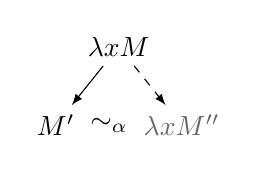
\begin{tikzpicture}[>=latex]
   \node (a) at (2,2) {$\lam x M$};
   \node (b) at (1.2,1) {$M'$};
   \node[opacity=0.6] (d) at (2.8,1) {$\lam x M''$};

   \draw [->] (a) -- (b) ;
   \draw [dashed,->] (a) -- (d) ;
   \path (b) --node{$\alpsym$} (d);
\end{tikzpicture}
\end{minipage}
\begin{minipage}{0.3\textwidth}
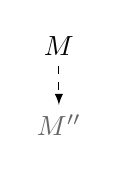
\begin{tikzpicture}[>=latex]
   \node (a) at (2,2) {$M$};
   \node[opacity=0.6] (b) at (2,1) {$M''$};

   \draw [dashed,->] (a) -- (b) ;
\end{tikzpicture}
\end{minipage}
  
\end{center}

\begin{proof}
We prove that $M'' = (y\ x) M'$\  satifies all conjunction assertions in the thesis.

As $\lam x M \p M'$\ by parallel elimination we know:
\begin{itemize}
\item $M'' = \lam y M'$
\item $\exists xs, \forall z \not\in xs, (x\ z)M \p (y\ z) M'$
\end{itemize}

Next prove the thesis conjunctions:

\begin{itemize}
\item
  \AxiomC{be $z \not\in xs \cup fv (\lam y M')$}
  \AxiomC{$\forall z \not\in xs, (x\ z)M \p (y\ z) M'$}
  \BinaryInfC{$(x\ z) M \p (y\ z) M'$}
  \LeftLabel{\p\ equiv.}
  \UnaryInfC{$(x\ z) (x\ z) M \p (x\ z) (y\ z) M'$}
  \LeftLabel{swap idem.}
  \UnaryInfC{$ M \p (x\ z) (y\ z) M'$}
  \AxiomC{$x \# \lam y M'$}
  \AxiomC{$z \not\in fv (\lam y M')$}
  \UnaryInfC{$z \# \lam y M'$}
  \BinaryInfC{$(x\ z) (y\ z) M' \alpsym (x\ y) M'$}   
  \LeftLabel{lem.\ref{prightalpha}}
  \BinaryInfC{$M \p (x\ y) M'$}   
  \DisplayProof

\item
  \AxiomC{$\lam x M \p \lam y M'$}
  \AxiomC{$\lam y M' \alpsym \lam x ((x\ y) M')$}
  \LeftLabel{lem.\ref{prightalpha}}
  \BinaryInfC{$\lam x M \p \lam x ((x\ y) M')$}   
  \DisplayProof

\item
  \AxiomC{$x \# \lam x M$}
  \AxiomC{$\lam x M \p \lam y M'$}
  \LeftLabel{lem.\ref{pfresh}}
  \BinaryInfC{$x \# \lam y M'$}
  \UnaryInfC{$\lam y M' \alpsym \lam x ((y\ x) M')$}
  \DisplayProof

\end{itemize}
\end{proof}

\begin{lem}[Parallel relation $\beta$-elimination] \
\label{betaelim}

\begin{center}
  \AxiomC{$\lam x M \p \lam y M'\quad N \p N' \quad M' [ y := N' ] \alpsym P$}
  \LeftLabel{\p$\beta$}
  \UnaryInfC{$(\lam x M) N \p P$}
  \DisplayProof
\end{center}  
  \[ \Downarrow \]
  \[ (\exists M'')( \lam x M \p \lam x M'' , M'' [x := N'] \alpsym P) \]

\end{lem} 

\begin{center}
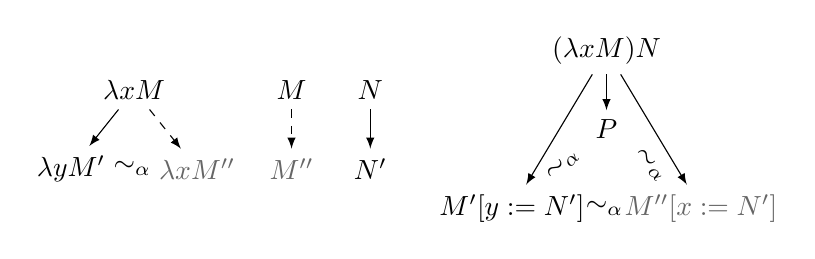
\begin{tikzpicture}[>=latex]
   \node (a) at (2,2) {$\lam x M$};
   \node (b) at (1.2,1) {$\lam y M'$};
   \node[opacity=0.6] (d) at (2.8,1) {$\lam x M''$};

   \node (g) at (4,2) {$M$};
   \node[opacity=0.6] (h) at (4,1) {$M''$};

   \node (e) at (5,2) {$N$};
   \node (f) at (5,1) {$N'$};

   \node (l) at (8,2.5) {$(\lam x M) N$};
   \node (i) at (8,1.5) {$P$};
   \node (j) at (6.8,0.5) {$M'[y:=N']$};
   \node[opacity=0.6] (k) at (9.2,0.5) {$M''[x:=N']$};

   \draw [->] (a) -- (b) ;
   \draw [->] (e) -- (f) ;
   \draw [dashed,->] (g) -- (h) ;
   \draw [dashed,->] (a) -- (d) ;
   \path (b) --node{$\alpsym$} (d);

   \draw [->] (l) -- (i) ;
   \draw [->] (l) -- (j) ;
   \draw [->] (l) -- (k) ;
   \path (i) --node[rotate=45]{$\alpsym$} (j);
   \path (i) --node[rotate=-45]{$\alpsym$} (k);
   \path (j) --node{$\alpsym$} (k);
\end{tikzpicture}
\end{center}


\begin{proof}
We prove that $M'' = (y\ x) M'$\  satifies the thesis:

\begin{itemize}
\item 
  \AxiomC{$\lam x M \p \lam y M'$}
  \AxiomC{$x \# \lam x M$}
  \AxiomC{$\lam x M \p \lam y M'$}
  \LeftLabel{lem.\ref{pfresh}}
  \BinaryInfC{$x \# \lam y M'$}
  \UnaryInfC{$\lam y M' \alpsym \lam x ((x\ y) M')$}
  \LeftLabel{lem.\ref{prightalpha}}
  \BinaryInfC{$\lam x M \p \lam x ((y\ x) M')$}   
  \DisplayProof
\item

\[ \begin{array}{lcl}
      ((y\ x) M') [x := N'] &\alpsym& \text{} \\
      ((x\ y) M') [x := N'] &\alpsym& \text{lemma~\ref{pequiv}(proved by alpha induction) using as } x \# \lam y M'  \\
      M' [y := N'] &\alpsym& \text{hypothesis} \\
      P
   \end{array} \]

\end{itemize}
\end{proof}

\section{Binder Relation}

\begin{minipage}{0.2\linewidth}
  \AxiomC{$\quad$}   \LeftLabel{\ninb v} \UnaryInfC{$x \ninb y$} \DisplayProof
\end{minipage}
\begin{minipage}{0.4\linewidth}
  \AxiomC{$x \ninb M$} 
  \AxiomC{$x \ninb N$}
  \LeftLabel{\ninb a}
  \BinaryInfC{$x \ninb M N$} \DisplayProof
\end{minipage}
\begin{minipage}{0.4\linewidth}
  \AxiomC{$x \neq y$}
  \AxiomC{$x \ninb M$}
  \LeftLabel{\ninb \lam}
  \BinaryInfC{$x  \ninb  \lambda y M$} \DisplayProof
\end{minipage}

\section{Another Alpha Primitive Induction Principle}
\label{sec:alphaprinciple}

If for some predicate $P$\ over terms  exists a finite set of atoms $A$\ then:

\[ \left.
  \begin{array}{lc}
    P\ \alpha\text{-compatible} & \wedge \\
    \forall a, P(a) & \wedge\\
    \forall M\ N, (\forall b \in A, b \ninb M N) \wedge P(M) \wedge P(N)  \Rightarrow P (M N) & \wedge \\    
    \forall M\ a,\ (\forall b \in A, b \ninb \lam a M) \wedge P(M)   \Rightarrow P (\lam a M) \\    
  \end{array} \right\} \Rightarrow \forall M, P(M)
\]

As in Barendregt convention, this induction principle enable us to assume binders position fresh enough from a given finite context of variables $A$ through the entire term induction (not only in the abstraction case). The following results uses this principle to avoid some binders in the $\beta$ case of the application.

\begin{lem}[Parallel relation substitution lemma]
\label{psubst}
\[ M \p M' \wedge N \p N'  \Rightarrow M [ x := N ] \p M' [ x := N' ] \]
\end{lem}

\begin{proof}
  Uses previously introduced \alp\ induction principle gave in~\ref{sec:alphaprinciple} over $M$\ term. Given some $N,N'$\ terms such that $N \p N'$ , and $x$\ atom, we define the following predicate over terms:

\[ P(M) \equiv \forall M', M \p M' \Rightarrow M [ x := N ] \p M' [ x := N' ] \]

  Next we prove that $P$ is \alp-compatible, that is,  $P(M) \wedge M \alpsym N \Rightarrow P(N)$. 
  
  \AxiomC{$M \alpsym N$} 
  \AxiomC{$N \p M'$} 
  \LeftLabel{lem.~\ref{pleftalpha}}
  \BinaryInfC{$M \p M'$}
  \AxiomC{$N \p N'$} 
  \LeftLabel{P(M)}
  \BinaryInfC{$M [ x := N ] \p M' [ x := N' ]$}
  \AxiomC{$M \alpsym N$} 
  \LeftLabel{subst.lemma}
  \UnaryInfC{$M [ x := N ] \equiv N [ x := N ]$}
  \LeftLabel{congruence}
  \BinaryInfC{$N [ x := N ] \p M' [ x := N' ]$}
  \DisplayProof
  
 We take as $\{x \} \cup fv(N) \cup fv(N')$\ the set of binders to avoid in the \alp-induction.

  \begin{itemize}
  \item[var case:] $\forall a, P(a)$
    \begin{itemize}
      \item[$x \equiv a$ subcase:] $x [x := N ] \equiv N \p N' \equiv x [ x := N' ]$
      \item[$x \not\equiv a$ subcase:]  $a [x := N ] \equiv a \p a \equiv a [ x := N' ]$
    \end{itemize}
  \item[app. case:] $\forall P\ Q, (\forall b \in \{x \} \cup fv(N) \cup fv(N'), b \ninb P Q) \wedge P(P) \wedge P(Q)  \Rightarrow P (P Q)$
    \begin{itemize}
      \item[\p a subcase:] 
        Hypotheses:                 
        \begin{minipage}{0.45\linewidth}
          \AxiomC{$P \p P'$} \AxiomC{$Q \p Q'$} \LeftLabel{\p a}
          \BinaryInfC{$P Q \p P' Q'$} \DisplayProof
        \end{minipage}
        Thesis:
        \begin{minipage}{0.5\linewidth}
          $(P Q) [x := N ] \p (P' Q') [x := N']$
        \end{minipage}
                      
          \AxiomC{$P \p P'$}
          \LeftLabel{$P(P)$}
          \UnaryInfC{$P [x := N] \p P' [x := N']$}
          \AxiomC{$Q \p Q'$}
          \LeftLabel{$P(Q)$}
          \UnaryInfC{$Q [x := N] \p Q' [x := N']$}
          \LeftLabel{\p a}
          \BinaryInfC{$(P Q) [x := N] \p (P' Q') [x := N']$} 
          \DisplayProof
 
          
              
      \item[$\beta$\ subcase:] \
        Hypotheses:
        \begin{minipage}{0.8\linewidth}
          \AxiomC{$\lam y P \p \lam z P'$} 
          \AxiomC{$Q \p Q'$}
          \AxiomC{$ P' [z:=Q'] \alpsym R$}
          \LeftLabel{\p $\beta$}
          \TrinaryInfC{$(\lam y P) Q \p R $} \DisplayProof
        \end{minipage}
        Thesis:
        \begin{minipage}{0.5\linewidth}
          $((\lam y P) Q) [x := N ] \p R [x := N']$
        \end{minipage}

\vspace{2mm}

        \AxiomC{$(\lam y P) Q \p R $}
        \LeftLabel{lem.~\ref{betaelim}} 
        \UnaryInfC{$\exists P'', \lam y P \p \lam y P'' \wedge P''[y:=Q'] \alpsym R$} 
        \DisplayProof

\vspace{2mm}
%        As $\forall b \in \{x \} \cup fv(N) \cup fv(N'), b \ninb (\lam y P) Q)$\ we have that $y \not\in \{x\} \cup fv(N)$\ and $y \not\in \{x\} \cup fv(N')$.

        \AxiomC{$\forall b \in \{x \} \cup fv(N) \cup fv(N'), b \ninb (\lam y P) Q$}
        \UnaryInfC{$y \not\in \{x\} \cup fv(N)$}
        \UnaryInfC{$ (\lam y P) [x := N]) \alpsym \lam y (P [x := N]) $}
        \DisplayProof

        Analog

        \AxiomC{$\forall b \in \{x \} \cup fv(N) \cup fv(N'), b \ninb (\lam y P) Q$}
        \UnaryInfC{$y \not\in \{x\} \cup fv(N')$}
        \UnaryInfC{$ (\lam y P'') [x := N'] \alpsym \lam y (P'' [x := N']) $}
        \DisplayProof

        So

        \AxiomC{$ (\lam y P) [x := N]) \alpsym \lam y (P [x := N]) $}
        \AxiomC{$Q [x:=N] \alpsym Q [x:=N]$}
        \LeftLabel{$\alpsym$a}
        \BinaryInfC{($(\lam y P) [x := N]) (Q [x:=N]) \alpsym (\lam y (P [x := N])) (Q [x:=N])$ }
        \UnaryInfC{$((\lam y P) Q) [x:=N] \alpsym (\lam y (P [x := N])) (Q [x:=N])$ }
        \DisplayProof

        Finally,

        %%\BinaryInfC{$\lam y (P [x := N]) \p (\lam y P'') [x := N']$}

        \AxiomC{$\lam y P \p \lam y P''$}
        \LeftLabel{$P(\lam y P)$}
        \UnaryInfC{$
          \begin{array}{c}
              (\lam y P) [x := N] 
            \p \\
            \begin{array}{c}
             (\lam y P'') [x := N'] \\
            \end{array}
          \end{array}$}
        \UnaryInfC{$
          \begin{array}{c}
            \lam y (P [x := N])  \p \\ \lam y (P'' [x := N'])
          \end{array}$}
        \AxiomC{$Q \p Q'$}
        \LeftLabel{$P(Q)$}
        \UnaryInfC{$
          \begin{array}{c}
            Q [x := N]  \p \\ Q' [x := N']
          \end{array}$}
        \AxiomC{$y \not\in \{x\} \cup fv(N')$}
        \UnaryInfC{$
          \begin{array}{c}
            P'' [x := N'] [y := Q' [x := N']] \alpsym \\
            P'' [y := Q' ][x := N']  \equiv  \\
            R [x := N']
          \end{array}$}
        \LeftLabel{$\p\beta$}
        \TrinaryInfC{$\underbrace{(\lam y (P [x := N])) (Q [x := N])}_{\alpsym ((\lam y P) Q) [x := N ]} \p  R [x := N']$}
        \DisplayProof        


    \end{itemize}
  \item[\lam\ case:] $\forall M\ a,\ (\forall b \in \{x \} \cup fv(N) \cup fv(N'), b \ninb \lam a M) \wedge P M   \Rightarrow P (\lam a M) $

        \begin{minipage}{0.4\linewidth}
          Hypotheses: $\lam y P \p Q $
        \end{minipage}
        \begin{minipage}{0.6\linewidth}
          Thesis: $(\lam y P) [x := N ] \p Q [x := N']$
        \end{minipage}

        \AxiomC{$(\lam y P) \p Q $}
        \LeftLabel{lem.~\ref{lamelim}} 
        \UnaryInfC{$\exists Q', P \p Q' \wedge \lam y P \p \lam y Q' \wedge Q \alpsym \lam y Q'$} 
        \DisplayProof

\vspace{2mm}
        \AxiomC{$y \not\in \{x\} \cup fv(N)$}         
        \UnaryInfC{$(\lam y P) [x:=N]) \alpsym \lam y (P [x:=N])$}
        \AxiomC{$P \p Q' $}         
        \LeftLabel{$P(P)$}         
        \UnaryInfC{$P [x:=N] \p Q' [x:=N']$}
        \UnaryInfC{$\lam y (P [x:=N]) \p \lam y (Q' [x:=N'])$}
        \BinaryInfC{$(\lam y P) [x:=N] \p \lam y (Q' [x:=N'])$}
        \AxiomC{$y \not\in \{x\} \cup fv(N')$}         
        \UnaryInfC{$
          \begin{array}{c}
            \lam y (Q' [x:=N']) \alpsym \\ (\lam y Q') [x:=N']
          \end{array}$}
        \BinaryInfC{$(\lam y P) [x:=N] \p \underbrace{(\lam y Q') [x:=N']}_{\equiv Q[x:=N']\ \text{as}\ Q \alpsym \lam y Q'}$}
        \DisplayProof


        
  \end{itemize}
\end{proof}


  \begin{lem}[Diamond property of parallel relation]
    \label{pdiamond}

    \begin{minipage}{0.7\linewidth}
    $ M \p N \wedge M \p P \Rightarrow \exists Q, N \p Q \wedge P \p  Q $
  \end{minipage}

  \begin{center}

    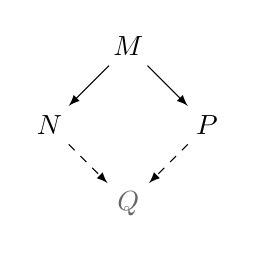
\begin{tikzpicture}[>=latex]  
   \node (a) at (2,2) {$M$};
   \node (b) at (1,1) {$N$};
   \node (c) at (3,1) {$P$};
   \node[opacity=0.6] (d) at (2,0) {$Q$};

   \draw [->] (a) -- (b) ;
   \draw [->] (a) -- (c) ;
   \draw [dashed,->] (b) -- (d) ;
   \draw [dashed,->] (c) -- (d) ;
 \end{tikzpicture}

  \end{center}




\end{lem}


\begin{proof}
  Induction on the $M$\ term.

  \begin{itemize}
  \item[var case:] Direct.
  \item[app. case:] Cases on both parallel reductions.

    \begin{itemize}
    \item[\p a-\p a subcase:] 
        Hypotheses:                 
        \begin{minipage}{0.45\linewidth}
          \AxiomC{$M \p N$} \AxiomC{$M' \p N'$} \LeftLabel{\p a}
          \BinaryInfC{$M M' \p N N'$} \DisplayProof
        \end{minipage}
        \begin{minipage}{0.45\linewidth}
          \AxiomC{$M \p P$} \AxiomC{$M' \p P'$} \LeftLabel{\p a}
          \BinaryInfC{$M M' \p  P P'$} \DisplayProof
        \end{minipage}

        Thesis:
        \begin{minipage}{0.5\linewidth}
          $\exists Q, N N' \p Q \wedge P P' \p Q$
        \end{minipage}

        \AxiomC{$M \p N$}
        \AxiomC{$M \p P$}
        \LeftLabel{ih}
        \BinaryInfC{$\exists Q, N \p Q \wedge P \p Q$}
        \AxiomC{$M' \p N'$}
        \AxiomC{$M' \p P'$}
        \LeftLabel{ih}
        \BinaryInfC{$\exists Q', N' \p Q' \wedge P' \p Q'$}
        \LeftLabel{\p a}
        \BinaryInfC{$\exists (Q Q'),N N'\p Q Q'  \wedge P P' \p Q Q'$}
        \DisplayProof
        
    \item[\p $\beta$-\p $\beta$\ subcase:] 
        Hypotheses:
        \begin{minipage}{0.8\linewidth}
          \AxiomC{$\lam x M \p \lam y N'$} 
          \AxiomC{$M' \p N''$}
          \AxiomC{$ N' [y:=N''] \alpsym N$}
          \LeftLabel{\p $\beta$}
          \TrinaryInfC{$(\lam x M) M' \p N $} \DisplayProof
        \end{minipage}

        \begin{minipage}{0.8\linewidth}
          \AxiomC{$\lam x M \p \lam z P'$} 
          \AxiomC{$M' \p P''$}
          \AxiomC{$ P' [z:=P''] \alpsym P$}
          \LeftLabel{\p $\beta$}
          \TrinaryInfC{$(\lam x M) M' \p P $} \DisplayProof
        \end{minipage}

        Thesis:
        \begin{minipage}{0.5\linewidth}
          $\exists Q, N \p Q \wedge P \p Q$
        \end{minipage}

        \AxiomC{$(\lam x M) M' \p N $}
        \LeftLabel{lem.~\ref{betaelim}} 
        \UnaryInfC{$\exists N''', \lam x M \p \lam x N''' \wedge N'''[x:=N''] \alpsym N$} 
        \DisplayProof

\vspace{2mm}

        \AxiomC{$(\lam x M) M' \p P $}
        \LeftLabel{lem.~\ref{betaelim}} 
        \UnaryInfC{$\exists P''', \lam x P \p \lam x P''' \wedge P'''[x:=P''] \alpsym P$} 
        \DisplayProof

\vspace{2mm}

        \AxiomC{$\lam x M  \p \lam x N''' $}
        \AxiomC{$\lam x M  \p \lam x P''' $}
        \LeftLabel{ih} 
        \BinaryInfC{$\exists R, \lam x N''' \p R \wedge \lam x P''' \p S $} 
        \DisplayProof

\vspace{2mm}

        \AxiomC{$M'  \p N'' $}
        \AxiomC{$M' \p P'' $}
        \LeftLabel{ih} 
        \BinaryInfC{$\exists S, N'' \p S \wedge P'' \p S $} 
        \DisplayProof

\vspace{2mm}

        \AxiomC{$\lam x N''' \p R $}
        \LeftLabel{lem.~\ref{lamelim}} 
        \UnaryInfC{$\exists R', N''' \p R' \wedge \lam x N''' \p \lam x R' \wedge R \alpsym \lam x R'$} 
        \DisplayProof

\vspace{2mm}

        \AxiomC{$\lam x P''' \p R $}
        \LeftLabel{lem.~\ref{lamelim}} 
        \UnaryInfC{$\exists R'', P''' \p R'' \wedge \lam x P''' \p \lam x R'' \wedge R \alpsym \lam x R''$} 
        \DisplayProof

\vspace{2mm}

        Finally,

        $\exists R' [x:=S], N \p R' [x:=S] , P \p R' [x:=S]$

        Because:

        \AxiomC{$N \alpsym N'''[x:=N'']$}        
        \AxiomC{$N''' \p R'$}
        \AxiomC{$N'' \p S$}
        \LeftLabel{lemma~\ref{psubst}}
        \BinaryInfC{$N'''[x:=N''] \p R'[x:=S] $}
        \BinaryInfC{$N \p R[x:=S] $}
        \DisplayProof

        \AxiomC{$P \alpsym P'''[x:=P'']$}        
        \AxiomC{$P''' \p R''$}
        \AxiomC{$R \alpsym \lam x R'$}
        \AxiomC{$R \alpsym \lam x R''$}
        \BinaryInfC{$R'' \alpsym R'$}
        \BinaryInfC{$P''' \p R'$}
        \AxiomC{$P'' \p S$}
        \LeftLabel{lemma~\ref{psubst}}
        \BinaryInfC{$P'''[x:=P''] \p R'[x:=S] $}
        \BinaryInfC{$P \p R'[x:=S] $}
        \DisplayProof

    \item[\p a-\p $\beta$\ subcase:] 
      Hypotheses:                 
        \begin{minipage}{0.45\linewidth}
          \AxiomC{$\lam x M \p N'$} \AxiomC{$M' \p N''$} \LeftLabel{(\p a)}
          \BinaryInfC{$(\lam x M) M' \p  N' N'' $} \DisplayProof
        \end{minipage}

        \begin{minipage}{0.8\linewidth}
          \AxiomC{$\lam x M \p \lam y P'$} 
          \AxiomC{$M' \p P''$}
          \AxiomC{$ P' [y:=P''] \alpsym P$}
          \LeftLabel{(\p $\beta$)}
          \TrinaryInfC{$(\lam x M) M' \p P $} \DisplayProof
        \end{minipage}

        Thesis:
        \begin{minipage}{0.5\linewidth}
          $\exists Q, N' N'' \p Q \wedge P \p Q$
        \end{minipage}

        Applying \lam\ and $\beta$\ elimination.

        \AxiomC{$\lam x M \p N' $}
        \LeftLabel{lem.~\ref{lamelim}} 
        \UnaryInfC{$\exists N''', M \p N''' \wedge \lam x M \p \lam x N''' \wedge  N' \alpsym \lam x N'''$}
        \DisplayProof

        \AxiomC{$(\lam x M) M' \p P $}
        \LeftLabel{lem.~\ref{betaelim}} 
        \UnaryInfC{$\exists P''', \lam x M \p \lam x P''' \wedge P'''[x:=P''] \alpsym P$} 
        \DisplayProof

        Applying inductive hypothesis.

        \begin{minipage}{0.5\linewidth}
          \AxiomC{$\lam x M \p \lam x N'''$}
          \AxiomC{$\lam x M \p \lam x P'''$} \LeftLabel{ih}
          \BinaryInfC{$\exists Q, \lam x N''' \p Q \wedge \lam x P''' \p Q$}
          \DisplayProof
        \end{minipage}

        \begin{minipage}{0.5\linewidth}
          \AxiomC{$M' \p N''$}
          \AxiomC{$M' \p P''$} \LeftLabel{ih}
          \BinaryInfC{$\exists R, N'' \p R \wedge P'' \p R$}
          \DisplayProof
        \end{minipage}
        
        Applying $\lam$-elimination again.

        \AxiomC{$\lam x N''' \p Q $}
        \LeftLabel{lem.~\ref{lamelim}} 
        \UnaryInfC{$\exists S', N''' \p S' \wedge \lam x N''' \p \lam x S' \wedge  Q \alpsym \lam x S'$}
        \DisplayProof

        \AxiomC{$\lam x P''' \p Q $}
        \LeftLabel{lem.~\ref{lamelim}} 
        \UnaryInfC{$\exists S'', P''' \p S'' \wedge \lam x P''' \p \lam x S'' \wedge  Q \alpsym \lam x S''$}
        \DisplayProof

        Finally $\exists S' [x:=R], N' N'' \p S' [x:=R] \wedge P \p S' [x:=R]$ as proved next.

        \AxiomC{$N' \alpsym \lam x N'''$}
        \AxiomC{$N'' \alpsym N''$}
        \LeftLabel{\p a} 
        \BinaryInfC{$N' N'' \alpsym (\lam x N''') N''$}
        \AxiomC{$\lam x N''' \p \lam x S'$}
        \AxiomC{$N'' \p R$}
        \LeftLabel{\p $\beta$} 
        \BinaryInfC{$(\lam x N''') N'' \p S' [x:=R]$}
        \LeftLabel{lem.} 
        \BinaryInfC{$N' N'' \p S'[x:=R]$}
        \DisplayProof


        \AxiomC{$P \alpsym P'''[x:=P'']$}        
        \AxiomC{$P''' \p S''$}
        \AxiomC{$Q \alpsym \lam x S'$}
        \AxiomC{$Q \alpsym \lam x S''$}
        \BinaryInfC{$S'' \alpsym S'$}
        \BinaryInfC{$P''' \p S'$}
        \AxiomC{$P'' \p R$}
        \LeftLabel{lemma~\ref{psubst}}
        \BinaryInfC{$P'''[x:=P''] \p S'[x:=R] $}
        \BinaryInfC{$P \p S'[x:=R] $}
        \DisplayProof

    \item[\p $\beta$-\p a\ subcase:] Analog to previous one.

    \end{itemize}
  \item[\lam\ case:] \
        \begin{minipage}{0.5\linewidth}
          Hypotheses: $\lam y M \p N \wedge \lam y M \p P$
        \end{minipage}
        \begin{minipage}{0.5\linewidth}
          Thesis: $\exists Q, N \p Q \wedge P \p Q$
        \end{minipage}

        \AxiomC{$(\lam y M) \p N $}
        \LeftLabel{lem.~\ref{lamelim}} 
        \UnaryInfC{$\exists N', M \p N' \wedge  N \alpsym \lam y N'$}


        \AxiomC{$(\lam y M) \p P $}
        \LeftLabel{lem.~\ref{lamelim}} 
        \UnaryInfC{$\exists P', M \p P' \wedge  P \alpsym \lam y P'$}
        \LeftLabel{ih} 
        \BinaryInfC{$\exists Q, N' \p Q \wedge P' \p Q$}
        \UnaryInfC{$\exists \lam y Q,\lam y N' \p \lam y Q \wedge \lam y P' \p \lam y Q$}
        \LeftLabel{lem.\ref{pleftalpha}} 
        \UnaryInfC{$\exists \lam y Q,N \p \lam y Q \wedge P \p \lam y Q$}
        \DisplayProof

  \end{itemize}
\end{proof}
  


\end{document}